\documentclass{article}
\usepackage{graphicx}
\begin{document}
\title{Gas Turbine Propulsion Toolbox: User Manual}
\author{Christopher Chinske}
\date{February 21, 2020}
\maketitle

Copyright 2016 Christopher Chinske.  This work is licensed under the
Creative Commons Attribution-ShareAlike 4.0 International License. To
view a copy of this license, visit
http://creativecommons.org/licenses/by-sa/4.0/ or send a letter to
Creative Commons, PO Box 1866, Mountain View, CA 94042, USA.

\section{Introduction}
The Gas Turbine Propulsion Toolbox (GTPT) is a collection of programs
that can be used to study gas turbine engine performance.  The
programs are implemented as GNU Octave functions and scripts.
However, the programs should run correctly in MATLAB.

GTPT is based on the engine models contained in
\emph{Aerothermodynamics of Gas Turbine and Rocket Propulsion} by
Gordon C. Oates.  GTPT reproduces some of the functionality of the
Engine Cycle Analysis Program (ECAP) and the Engine Off-Design
Performance Program (EOPP), which are distributed with the book by
Oates.

GTPT also includes example code for engine performance modeling (EPM).
For example, if you know the specific fuel consumption for an engine
at a particular reference point, and you know the engine’s pressure
ratio and bypass ratio, then GTPT can be used to determine a feasible
set of parameters (e.g., component pressure ratios, polytropic
efficiencies, etc.) that match the engine’s known performance.  These
parameters can then be used in an engine performance model to estimate
the engine’s performance at an off-design point.

\section{How to Use This Manual}
Commands are in mono-spaced typeface.  For example:
\newline
\newline
\texttt{[f\_mdot, s, inputs] = ideal\_turbojet}
\newline
\newline
Commands that could have more than one form are shown as \texttt{<example>}
\newline
Arguments that are optional are shown as \texttt{[example]}

\section{Concept of Operations}
GTPT operations can be divided into four categories:
\begin{enumerate}
\item Ideal Cycle Analysis
\item Non-Ideal Cycle Analysis
\item Off-Design Performance
\item Engine Performance Modeling.
\end{enumerate}
In general, GTPT can be used to analyze turbojet and turbofan engines.

\begin{figure}[h]
  \centering
  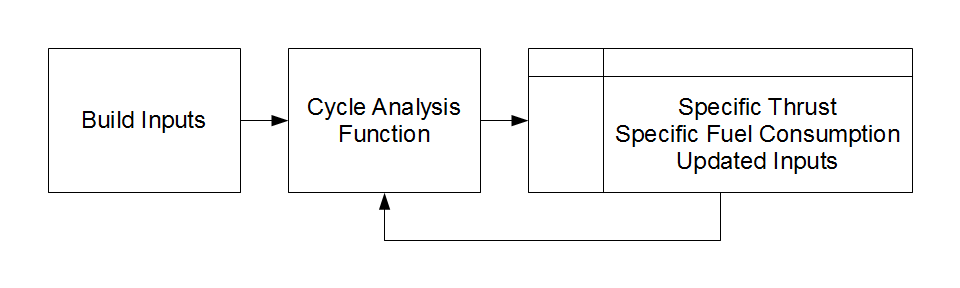
\includegraphics[width=4.25in]{figure-cycle-analysis-flowchart.png}
  \caption{General program flow}
  \label{fig:cycleflow}
\end{figure}

Figure \ref{fig:cycleflow} shows the general program flow for Ideal
Cycle Analysis, Non-Ideal Cycle Analysis, and Off-Design Performance.
The general process is as follows.
\begin{description}
\item[Build Inputs] The user builds a structure array where the fields
  of the structure array are the input parameters.  In many cases, the
  cycle analysis function will prompt the user for the input
  parameters if an input structure array is not provided as an
  argument to the function.  See ICD-GTPT-001 for a detailed
  description of the interfaces for each function.
\item[Cycle Analysis Function] The user calls the cycle analysis
  function.
\item[Output] In general, each cycle analysis function will output
  specific thrust and specific fuel consumption.  Some functions will
  output an updated input structure array.
\end{description}

\begin{figure}[h]
  \centering
  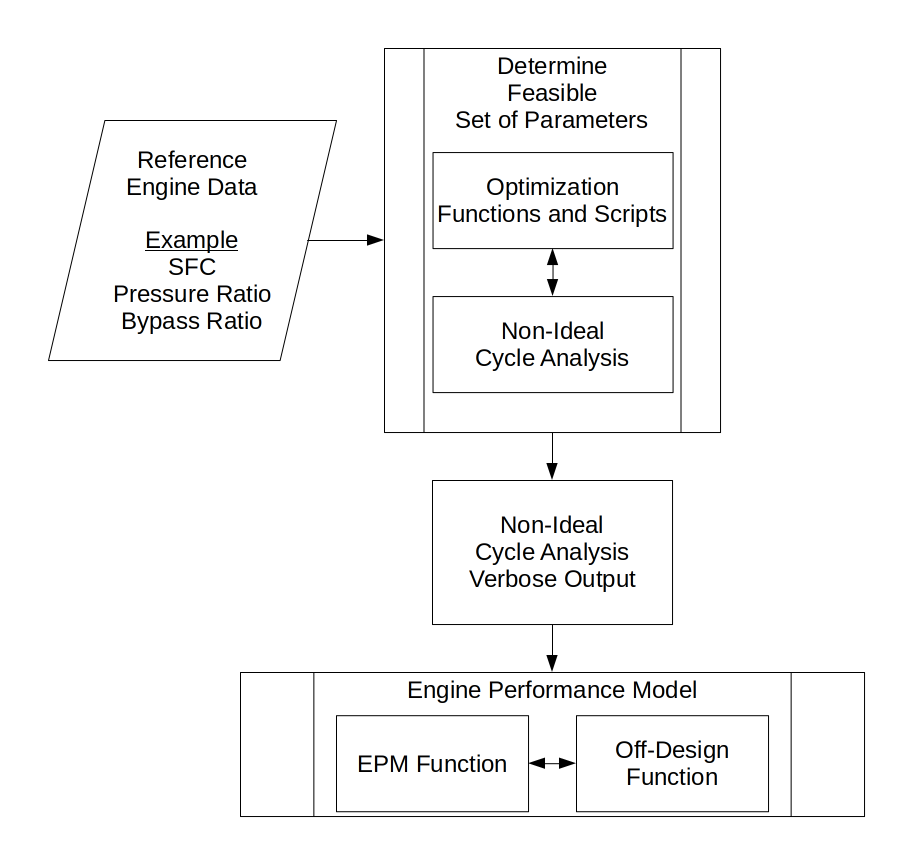
\includegraphics[width=4.25in]{figure-epm-flowchart.png}
  \caption{Engine performance modeling}
  \label{fig:epm}
\end{figure}

Figure \ref{fig:epm} shows the process for generating an engine
performance model based on limited engine reference data.  GTPT
includes example code for determining a feasible set of parameters and
for engine performance modeling.  First, optimization functions
interface with a non-ideal cycle analysis function to determine a
feasible set of parameters.  Then, these parameters are used to build
an engine performance model that interfaces with an off-design
performance function.

\section{Procedures}
\subsection{General}
To display a short message describing the calling syntax of a
function, type:
\newline
\newline
\texttt{help <function>}
\newline
\newline

Be sure that your load path is correctly configured.  In particular,
for engine performance modeling, the following directories must be on
your load path.
\begin{itemize}
\item optimize
\item epm
\end{itemize}

\subsection{Build Input Structure Array}
\subsubsection{General}
In many cases, the cycle analysis function will prompt you for the
input parameters if an input structure array is not provided as an
argument to the function.  For example:
\newline
\newline
\texttt{[f\_mdot, s, inputs] = ideal\_turbojet}
\newline
\newline
Alternatively, you can build an input structure array by typing:
\newline
\newline
\texttt{inputs = build\_inputs}
\newline
\newline

BUILD\_INPUTS may prompt you for inputs that do not apply to your
particular problem.  For example, bypass ratio is not required for an
analysis of a turbojet engine.

BUILD\_INPUTS\_OD\_TURBOJET and BUILD\_INPUTS\_OD\_TURBOFAN should be
used to build the input structure array for OD\_TURBOJET and
OD\_TURBOFAN, respectively.

Also, you may always choose to manually build the input structure
array.

\subsubsection{Vector Input}
In general, each input parameter is a single value.  However, one
input parameter may be a vector.  This allows computation of the
outputs (primarily specific thrust and specific fuel consumption) as a
function of an input variable.

\subsection{Ideal Cycle Analysis}
\begin{itemize}
\item Build the input structure array.
\item Call the ideal cycle analysis function.
\end{itemize}

\begin{tabular}{|l|} \hline
  \emph{List of Functions} \\ \hline
  IDEAL\_TURBOJET \\
  IDEAL\_TURBOJET\_AB \\
  IDEAL\_TURBOFAN \\
  IDEAL\_TURBOFAN\_AB \\
  IDEAL\_TURBOFAN\_MIXED \\ \hline
\end{tabular}

\subsection{Non-Ideal Cycle Analysis}
\begin{itemize}
\item Build the input structure array.
\item Call the non-ideal cycle analysis function.
\end{itemize}

\begin{tabular}{|l|} \hline
  \emph{List of Functions} \\ \hline
  NONIDEAL\_TURBOJET \\
  NONIDEAL\_TURBOFAN \\
  NONIDEAL\_TURBOFAN2 \\ \hline
\end{tabular}

\subsection{Off-Design Performance}
\begin{itemize}
\item Build the input structure array.
\item Call the off-design performance function.
\end{itemize}

\begin{tabular}{|l|} \hline
  \emph{List of Functions} \\ \hline
  OD\_TURBOJET \\
  OD\_TURBOFAN \\ \hline
\end{tabular}

\subsection{Engine Performance Modeling}
\begin{itemize}
\item Configure your load path
  \begin{itemize}
  \item \texttt{addpath optimize}
  \item \texttt{addpath epm}
  \end{itemize}
\item Create an optimization script based on optimize/s\_seek.m
  \begin{itemize}
  \item This script defines the lower bounds and upper bounds of the
    free (i.e., unknown) variables.
  \item The function SQP is used as the solver.
  \end{itemize}
\item Create an objective function based on optimize/phi.m
  \begin{itemize}
  \item This function defines the fixed (i.e., known) variables.
  \item This function calls a cycle analysis function.
  \item This function computes the absolute error between the output
    of the cycle analysis function and the known measure of
    performance.
  \item The absolute error is returned as the objective function to be
    minimized.
  \end{itemize}
\item Run the optimization script
\item Use the output from the optimization script to build an engine
  performance model based on epm/example\_epm.m
\end{itemize}

\end{document}
